% Lecture Template for ME3050 - Dynamic Modeling and Controls - Tennessee Technological University
% Spring 2024 - condensing and streamlining lectures by combining topics into a single PDF under the module name
% this will simplify file and link management as well as make lectures easier to use in class
% - added image/ to clean directory and reduce redundancy, specific to module for now  

% Module Name: - Frequency Response
% Topic 1 - Frequency Response of First Order Systems 
% Topic 2 - The Bode Diagram
% Topic 3 - Frequency Response of 2$^{nd}$ Order Systems
% Topic 4 - Resonance

\documentclass[fleqn]{beamer} % for presentation (has nav buttons at bottom)

%\usepackage{/home/tntech.edu/thill/courses/dmc/lectures/dmc_lectures}
%\usepackage{/home/thill/courses/dmc/lectures/dmc_lectures}
\usepackage{/mnt/c/Users/thill/Documents/courses/dmc/lectures/dmc_lectures}

\author{ME3050 - Dynamics Modeling and Controls}

\newcommand{\MNUM}{2\hspace{2mm}} % module number 
\newcommand{\moduletitle}{Frequency Response}

\newcommand{\sectionItitle}{Frequency Response of First Order Systems}
\newcommand{\sectionIItitle}{The Bode Diagram}
\newcommand{\sectionIIItitle}{Frequency Response of 2$^{nd}$ Order Systems}
\newcommand{\sectionIVtitle}{Resonance}

\newcommand{\sectionIsubsectionItitle}{Frequency Input Concept}
\newcommand{\sectionIsubsectionIItitle}{Complex Numbers Review}
\newcommand{\sectionIsubsectionIIItitle}{Frequency Response of First Order Systems}
\newcommand{\sectionIsubsectionIVtitle}{Graph of Frequency Response}

\newcommand{\sectionIIsubsectionItitle}{Review Frequency Response}
\newcommand{\sectionIIsubsectionIItitle}{Amplitude ratio in Decibels}
\newcommand{\sectionIIsubsectionIIItitle}{The Bode Diagram}
\newcommand{\sectionIIsubsectionIVtitle}{Frequency Response in MATLAB}

\newcommand{\sectionIIIsubsectionItitle}{Review Transfer Functions}
\newcommand{\sectionIIIsubsectionIItitle}{Frequency Response of Overdamped Systems}
\newcommand{\sectionIIIsubsectionIIItitle}{Frequency Response of Underdamped Systems}
\newcommand{\sectionIIIsubsectionIVtitle}{MATLAB Bode Plots}

\newcommand{\sectionIVsubsectionItitle}{Review 2$^{nd}$ Order Frequency Response}
\newcommand{\sectionIVsubsectionIItitle}{The Resonance Phenomenon}
\newcommand{\sectionIVsubsectionIIItitle}{The Resonance Frequency}
\newcommand{\sectionIVsubsectionIVtitle}{---}

\newcommand{\LT}{\mathcal{L}} % lagrangian

% custom box
\newsavebox{\mybox}

\title{Lecture Module - \moduletitle}

\date{Mechanical Engineering\vspc Tennessee Technological University}

\begin{document}

	\lstset{language=MATLAB,basicstyle=\ttfamily\small,showstringspaces=false}

	\frame{\titlepage \center\begin{framed}\Large \textbf{\moduletitle}\end{framed} \vspace{5mm}}

	% Module Outline
	\begin{frame} 
		\large \textbf{Lecture Module - \moduletitle} \vspace{3mm}\\

		\begin{itemize}
			\item Topic 1 - \hyperlink{sectionI}{\sectionItitle} \vspc % section I
			\item Topic 2 - \hyperlink{sectionII}{\sectionIItitle} \vspc % section II
			\item Topic 3 - \hyperlink{sectionIII}{\sectionIIItitle} \vspc % section III
			\item Topic 4 - \hyperlink{sectionIV}{\sectionIVtitle} \vspc % section IV
		\end{itemize}

	\end{frame}

	% section I
	\section{\sectionItitle}\label{sectionI}

		% section I Outline
		\begin{frame} 
			\large \textbf{Topic 1 - \sectionItitle} \vspace{3mm}\\

			\begin{itemize}
				\item \hyperlink{sectionIsubsectionI}{\sectionIsubsectionItitle} \vspc %  section I subsection I
				\item \hyperlink{sectionIsubsectionII}{\sectionIsubsectionIItitle} \vspc % section I subsection II
				\item \hyperlink{sectionIsubsectionIII}{\sectionIsubsectionIIItitle} \vspc % section I subsection III
				\item \hyperlink{sectionIsubsectionIV}{\sectionIsubsectionIVtitle} \vspc % section I subsection IV
			\end{itemize}
		\end{frame}
		
		% section I subsection I 
		\subsection{\sectionIsubsectionItitle}\label{sectionIsubsectionI}

			\begin{frame}
				\frametitle{\sectionIsubsectionItitle}
				\bigskip

					\small 
					The term {\bf frequency response} is used to describe a system's response to a periodic input. Frequency response analysis focuses on a system's response to {\it harmonic} input such as sines and cosines. The input (forcing) function is written below.\vspcc


					\begin{framed}
					\scalebox{1.25}{$f(t)=Asin\left(\omega t\right)$}\vspccc

					\renewcommand{\arraystretch}{1.5}
					\begin{tabular}{ccc}
					Amplitude of the Input, & \scalebox{1}{$A$} & \scalebox{1}{$ (N)$} \\
					Frequency of Input, &\scalebox{1}{$\omega$} &  \scalebox{1}{$(\frac{rad}{s})$}\\
					\end{tabular}
					\end{framed}

				\btVFill
			\end{frame}

			\begin{frame}
				\frametitle{\sectionIsubsectionItitle}
				\bigskip

				%\frametitle{Why Study Frequency Response?}
				\small
				 Why do we care about the way a system responds to harmonic excitation? Why is {\bf frequency analysis} important? \\
				\begin{itemize}
				\item
				\item
				\item
				\end{itemize}

				\vspace{3mm}What causes {\bf harmonic} (or sinusoidal) excitation in the real world? \\

				\begin{itemize}
				\item
				\item
				\item
				\end{itemize}
 
				\btVFill
			\end{frame}

			\begin{frame}
				\frametitle{\sectionIsubsectionItitle}
				\bigskip

				%\frametitle{Frequency Response and the Transfer Function}

				A linear, time-invariant (LTI) system has a {\bf transfer function} $T(s)$ that describes the {\bf input-output} relationship of the system. Under sinusoidal excitation (input) with frequency $\omega$ if the system is stable the transient affects in the response (output) will eventually disappear leaving the {\bf steady state sinusoidal response} of the same frequency as the input but with a phase shift w.r.t. the input.


				\btVFill
			\end{frame}

		



		% section I subsection II
		\subsection{\sectionIsubsectionIItitle}\label{sectionIsubsectionII}

			\begin{frame}
				\frametitle{\sectionIsubsectionIItitle}
				\bigskip

				%\frametitle{The Complex Plane}

				In an underdamped system the roots of the characteristic polynomial are complex. Before we proceed we need to review some rules of arithmetic and complex numbers. \vspc

				\begin{multicols}{2}
				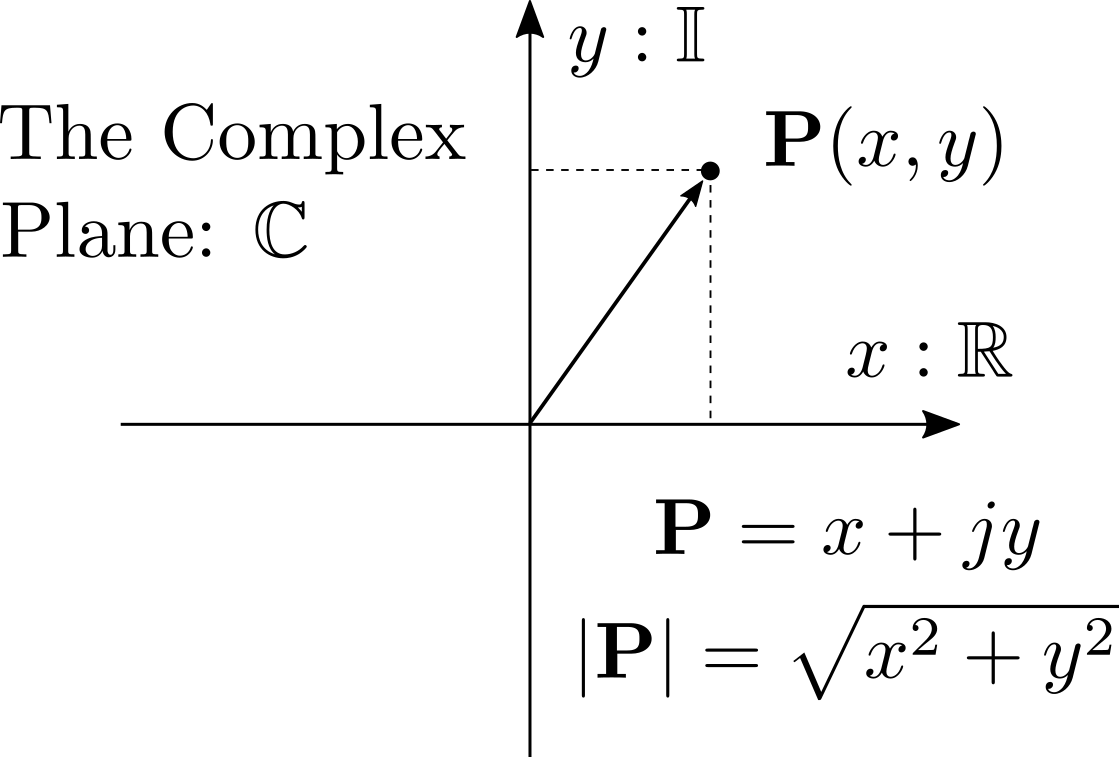
\includegraphics[scale=0.175]{images/lecture1_fig1.png}

				\small
				\hspccc Cartesian Representation:\vspc\hspccc\scalebox{.8}{$\mathbf{P}=x+jy$}\vspc
				\hspccc Polar Representation:\vspc\hspccc\scalebox{.8}{$\mathbf{P}=|\mathbf{P}|\angle\theta$}\vspc
				\hspccc Exponential Representation:\vspc\hspccc\scalebox{.8}{$\mathbf{P}=|\mathbf{P}|e^{j\theta}=|\mathbf{P}|\left(cos\theta+jsin\theta\right)$}\vspc
				\end{multicols}

				\btVFill
			\end{frame}

				%\btVFill
			\begin{frame}
				\frametitle{\sectionIsubsectionIItitle}
				\bigskip

				\frametitle{Complex Number Algebra}
 
				 Consider two points $\mathbf{P_1}$ and $\mathbf{P_2}$ on the complex plane. \vspc
				 
				 \scalebox{1}{$\mathbf{P_1}=x_1+jy_1$\hspc and \hspc$\mathbf{P_2}=x_2+jy_2$} \vspccc
				\renewcommand{\arraystretch}{1.75}
				 \begin{tabular}{cc}
				 Addition:& \scalebox{1}{$\mathbf{P_1}+\mathbf{P_2}=(x_1+x_2)+j(y_1+y_2)$}\\
				 Multiplication:& \scalebox{1}{$\mathbf{P_1P_2}=|\mathbf{P_1P_2}|\angle\left(\theta_1+\theta_2\right)$}\\
				 Division:&\scalebox{1}{$\frac{\mathbf{P_1}}{\mathbf{P_2}}=(x_1+x_2)+j(y_1+y_2)$}\\
				\end{tabular}
				
				\btVFill
			\end{frame}

		% section I subsection III
		\subsection{\sectionIsubsectionIIItitle}\label{sectionIsubsectionIII}
			\begin{frame} 
				\frametitle{\sectionIsubsectionIIItitle}
				\bigskip

				\frametitle{First Order Mass Damper}

				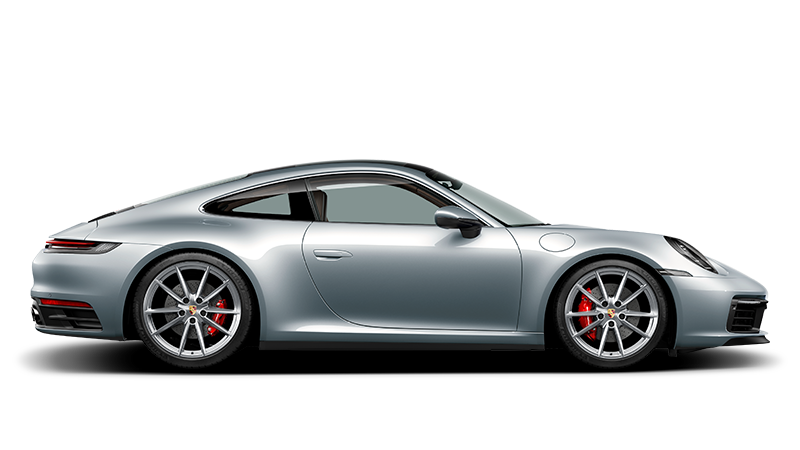
\includegraphics[scale=.15]{images/porsche.png}

				Consider our $1^{\underline{st}}$ order mass damper system. \vspc

				\scalebox{1}{$m\dot{v}+cv=f(t)$} \hspcc with a {\bf time constant} \scalebox{1}{$\tau=\frac{m}{c}$} \vspcc

				The system is commonly re-written as shown below. \vspc

				\scalebox{1}{$m\dot{v}+cv=f(t)\hspc\rightarrow\hspc\tau\dot{y}+y=f(t)$} \vspc

				\btVFill
			\end{frame}	

			\begin{frame} 
				\frametitle{\sectionIsubsectionIIItitle}
				\bigskip

				\frametitle{First Order Transfer Function}

				\small

				\scalebox{1}{$\tau\dot{y}+y=f(t)$} \vspcc

				Take the Laplace transform of the ODE. \vspcc

				\scalebox{1}{$\LT\{\tau\dot{y}+y\}=\LT\{f(t)\}$} \vspcc

				\scalebox{1}{$\tau\left(sY(s)+y_0)\right)+Y(s)=F(s)$}\hspccc The initial conditions are zero. \vspcc

				\begin{framed}
				\scalebox{1}{$T(s)=\frac{Y(s)}{F(s)}=\frac{1}{\tau s+1}$}\hspccc First Order Transfer Function
				\end{framed}

				This considers a {\it generalized} input function $f(t)$ and zero ICs.
				\btVFill
			\end{frame}	

		% section I subsection IV
		\subsection{\sectionIsubsectionIVtitle}\label{sectionIsubsectionIV}

			\begin{frame}
				\frametitle{\sectionIsubsectionIVtitle}
				\bigskip

				\frametitle{Sinusoidal Input Function}

				\small

				Our model is now excited by a sinusoidal input function. \vspc

				\scalebox{1}{$\tau\dot{y}+y=f(t)=Asin\left(\omega t\right)$} \vspc

				Take the Laplace transform. Then, solve for $Y(s)$ and expand.\vspc

				\scalebox{1}{$\tau sY(s)+Y(s)=\frac{A\omega}{s^2+\omega^2}$}  \vspc

				\scalebox{1}{$Y(s)=\frac{A\omega}{\left(s^2+\omega^2\right)\left(\tau s+1\right)}=\frac{C_1}{\tau s+1}+\frac{C_2s}{\left(s^2+\omega^2\right)}+\frac{C_3\omega}{\left(s^2+\omega^2\right)}$} \vspc

				Now solve for the coefficients.\vspc

				\scalebox{1}{$C_1=\frac{A\omega\tau^2}{1+\omega^2\tau^2}\hspccc,\hspc C_2=\frac{-A\omega\tau}{1+\omega^2\tau^2}\hspccc,\hspc C_3=\frac{A}{1+\omega^2\tau^2}$} \vspc

				Substituting and take the inverse Laplace transform. \vspc
				\scalebox{1}{$y(t)=\frac{A\omega\tau}{1+\omega^2\tau^2}\big( e^{\frac{-t}{\tau}}-cos\omega t+\frac{1}{\omega\tau}sin\omega t\big) $}
		
				\btVFill
			\end{frame}	

			\begin{frame}
				\frametitle{\sectionIsubsectionIVtitle}
				\bigskip

				\frametitle{Steady State Time Response}

				\small
				\scalebox{1}{$y(t)=\frac{A\omega\tau}{1+\omega^2\tau^2}\big( e^{\frac{-t}{\tau}}-cos\omega t+\frac{1}{\omega\tau}sin\omega t\big) $} \vspcc
				After some amount of time passes, the transient term will disappear leaving just the sinusoidal terms. \vspcc

				\scalebox{1}{$y(t)=\frac{A}{1+\omega^2\tau^2}\big(sin\omega t - \omega\tau cos\omega t\big) $} \vspccc
				This is re-written as a single sine term with a phase shift. \vspc

				\begin{framed}
				Steady State Frequency Response of First Order System\vspc
				\scalebox{1}{$y(t)=\frac{A}{\sqrt{1+\omega^2\tau^2}}sin\left(\omega t+\phi\right) \hspccc,\hspc \phi=-tan^{-1}\omega\tau$}
				\end{framed}

				\btVFill
			\end{frame}	

			\begin{frame}
				\frametitle{\sectionIsubsectionIVtitle}
				\bigskip
				\frametitle{Amplitude Ratio}

				\small

				\scalebox{1}{$y(t)=\frac{A}{\sqrt{1+\omega^2\tau^2}}sin\left(\omega t+\phi\right) \hspccc,\hspc \phi=-tan^{-1}\omega\tau$} \vspc

				Notice that the system responds at the same frequency as the input but with a different amplitude and a phase shift. The ratio of the response amplitude to the input amplitude is called the {\bf amplitude ratio, M}. \vspc

				\scalebox{1}{$M=\frac{\frac{A}{\sqrt{1+\omega^2\tau^2}}}{A}=\frac{1}{\sqrt{1+\omega^2\tau^2}}$} \vspc

				Fortunately we can find the {\bf amplitude ratio} and {\bf phase shift} directly from the transfer function. Recall the transfer function we derived. \vspc

				\scalebox{1}{$T(s)=\frac{1}{\tau s+1}$}\hspccc let \scalebox{1}{$s=j\omega\hspccc\implies\hspccc T(j\omega)=\frac{1}{\tau j\omega+1}$} \vspc

				\scalebox{1}{$|T(j\omega)|=\frac{|1|}{|\tau j\omega+1|}=\frac{1}{\sqrt{\left(\tau\omega\right)^2+1^2}}=\frac{1}{\sqrt{1+\tau^2\omega^2}}$} \hspccc \hspccc Look familiar? \vspc 

				\btVFill
			\end{frame}

			\begin{frame}
				\frametitle{\sectionIsubsectionIVtitle}
				\bigskip
				\frametitle{Phase Angle}		
				\small

				\scalebox{1}{$|T(j\omega)|=\frac{1}{\sqrt{1+\tau^2\omega^2}}=M(\omega)$}\vspc

				\scalebox{1}{$\angle T\left(j\omega\right)=\angle 1-\angle\left(1+j\omega\tau\right)=tan^{-1}\left(\frac{0}{1}\right)-tan^{-1}\left(\frac{\omega\tau}{1}\right)=$}\vspc
				\scalebox{1}{$-tan^{-1}\left(\omega\tau\right)=\phi(\omega)$}\vspcc

				Substitute $s=j\omega$ into the transfer function and solve for the magnitude and phase angle of this complex number which represent the magnitude ratio and phase shift. \vspc

				Therefore the steady state response is written as follows.  \vspc

				\scalebox{1}{$y_{ss}\left(t\right)=A|T\left(j\omega\right)|sin\left(\omega t+\angle T\left(j\omega\right)\right)=MAsin\left(\omega t+\phi\right)$}\vspcc

				Wasn't that fun? Can you believe we used to do that on the board?!?! \vspc

				\btVFill
			\end{frame}
	
	% Section II
	\section{\sectionIItitle}\label{sectionII}

		% section II Outline
		\begin{frame}
			\large \textbf{Topic 2 - \sectionIItitle} \vspace{3mm}\\

			\begin{itemize}
				\item \hyperlink{sectionIIsubsectionI}{\sectionIIsubsectionItitle} \vspc %  section II subsection I
				\item \hyperlink{sectionIIsubsectionII}{\sectionIIsubsectionIItitle} \vspc % section II subsection II
				\item \hyperlink{sectionIIsubsectionIII}{\sectionIIsubsectionIIItitle} \vspc % section II subsection III
				\item \hyperlink{sectionIIsubsectionIV}{\sectionIIsubsectionIVtitle} \vspc % section II subsection IV
			\end{itemize}

		\end{frame}

		% section II subsection I
		\subsection{\sectionIIsubsectionItitle}\label{sectionIIsubsectionI}

			\begin{frame}[label=sectionIIsubsectionI]
				\frametitle{\sectionIIsubsectionItitle}
				\bigskip

				\frametitle{Harmonic Input Function}

				\small 
				The term {\bf frequency response} is used to describe a system's response to a periodic input. Frequency response analysis focuses on a system's response to {\it harmonic} input such as sines and cosines. The input (forcing) function is written below.\vspcc

				\begin{framed}
				\scalebox{1.25}{$f(t)=Asin\left(\omega t\right)$}\vspccc

				\renewcommand{\arraystretch}{1.5}
				\begin{tabular}{ccc}
				Amplitude of the Input, & \scalebox{1}{$A$} & \scalebox{1}{$ (N)$} \\
				Frequency of Input, &\scalebox{1}{$\omega$} &  \scalebox{1}{$(\frac{rad}{s})$}\\
				\end{tabular}
				\end{framed}
				
				\btVFill
			\end{frame}

			\begin{frame}[label=sectionIIsubsectionI]
				\frametitle{\sectionIIsubsectionItitle}
				\bigskip

				\frametitle{First Order Frequency Response}

				\small

				The steady state response we derived is shown. Remember, after some amount of time passes, the transient term will disappear leaving just the sinusoidal terms. \vspc
				\begin{framed}
				\scalebox{1}{$y_{ss}\left(t\right)=A|T\left(j\omega\right)|sin\left(\omega t+\angle T\left(j\omega\right)\right)=MAsin\left(\omega t+\phi\right)$}\vspcc

				The amplitude ratio and phase shift can be found from $T(j\omega)$. \vspcc

				\scalebox{1}{$M(\omega)=|T(j\omega)|=\frac{1}{\sqrt{1+\tau^2\omega^2}}$}\vspc

				\scalebox{1}{$\phi(\omega)=\angle T\left(j\omega\right)=-tan^{-1}\left(\omega\tau\right)$}\vspc
				\end{framed}

				\btVFill
			\end{frame}

			\begin{frame}[label=sectionIIsubsectionI]
				\frametitle{\sectionIIsubsectionItitle}
				\bigskip

				\frametitle{Graph of Frequency Response}

				\small

				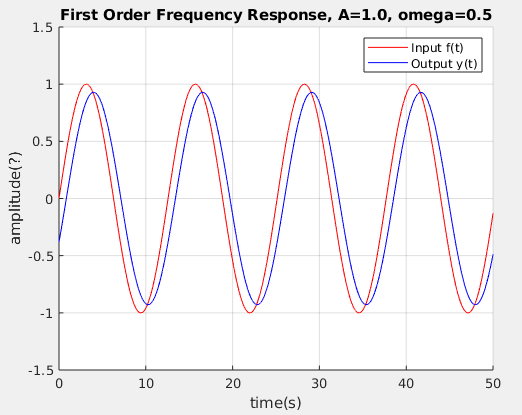
\includegraphics[scale=.275]{images/lecture1_fig6.png} \hspc 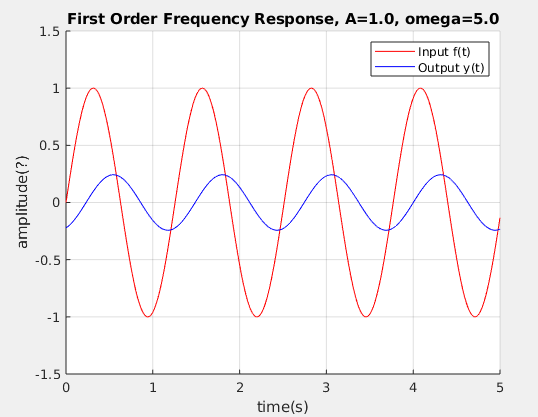
\includegraphics[scale=.275]{images/lecture1_fig5.png}  \vspc

				The amplitude of the response is determined by the input frequency. \vspc

				\btVFill
			\end{frame}


		% section II subsection II
		\subsection{\sectionIIsubsectionIItitle}\label{sectionIIsubsectionII}

			\begin{frame}

				\frametitle{\sectionIIsubsectionIItitle}
				\bigskip

				\frametitle{First Order Frequency Response}

				\small

				The steady state response we derived is shown. Remember, after some amount of time passes, the transient term will disappear leaving just the sinusoidal terms. \vspc
				\begin{framed}
				\scalebox{1}{$y_{ss}\left(t\right)=A|T\left(j\omega\right)|sin\left(\omega t+\angle T\left(j\omega\right)\right)=MAsin\left(\omega t+\phi\right)$}\vspcc

				The amplitude ratio and phase shift can be found from $T(j\omega)$. \vspcc

				\scalebox{1}{$M(\omega)=|T(j\omega)|=\frac{1}{\sqrt{1+\tau^2\omega^2}}$}\vspc

				\scalebox{1}{$\phi(\omega)=\angle T\left(j\omega\right)=-tan^{-1}\left(\omega\tau\right)$}\vspc
				\end{framed}

				\btVFill 
			\end{frame}

			\begin{frame}

				\frametitle{\sectionIIsubsectionIItitle}
				\bigskip


				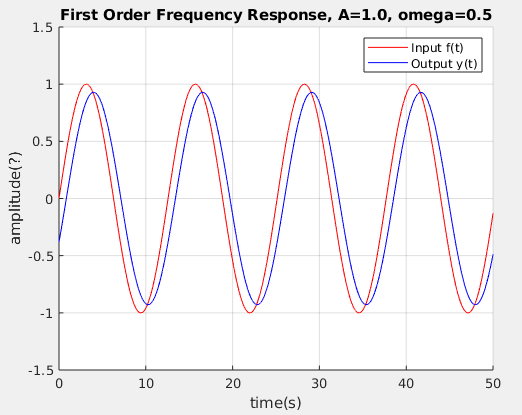
\includegraphics[scale=.275]{images/lecture1_fig6.png} \hspc 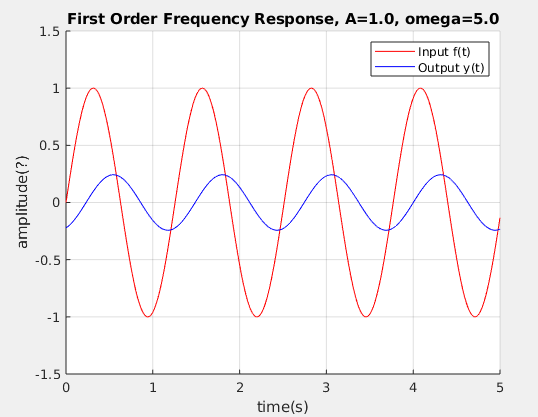
\includegraphics[scale=.275]{images/lecture1_fig5.png}  \vspc

				The amplitude of the response is determined by the input frequency. \vspc


				\btVFill 
			\end{frame}




		% section II subsection III
		\subsection{\sectionIIsubsectionIIItitle}\label{sectionIIsubsectionIII}

			\begin{frame}
				\frametitle{\sectionIIsubsectionIIItitle}
				\bigskip

				\frametitle{Dependence on Input Frequency}
				\begin{multicols}{2}

				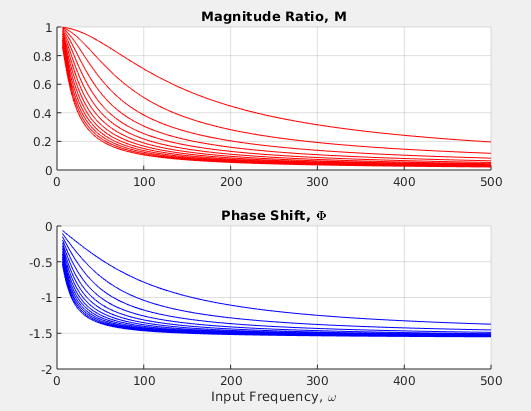
\includegraphics[scale=.27]{images/lecture2_fig2.png}

				You can see that the amplitude ratio decreases as the input frequency increases. The individual curves represent systems with different time constants. 

				\end{multicols}
	
				\btVFill 
			\end{frame}	


			\begin{frame}
				\frametitle{\sectionIIsubsectionIItitle}
				\bigskip

				\frametitle{Review Properties of Logarithms}

				\underline{Basic Properties of Logarithms:}\vspc
				\renewcommand{\arraystretch}{1.5}
				\begin{tabular}{cc}
				Multiplication&\scalebox{1}{$log(pq)=log(p)+log(q) $} \\
				Division&\scalebox{1}{$log(\frac{x}{y})=log(x)-log(y)$} \\
				Power&\scalebox{1}{$log(x^n)=nlog(x)$}\\
				\end{tabular}

				\underline{Units of Decibels for Magnitude:}\vspc
				\scalebox{1}{$m(dB)=10log(M^2)=20log(M)$ \hspccc convert back: \hspccc $M=10^{\frac{m(dB)}{20}}$}\vspc

				\small
				Decibel (dB), unit for expressing the ratio between two physical quantities, usually amounts of acoustic or electric power, or for measuring the relative loudness of sounds. One decibel (0.1 bel) equals 10 times the common logarithm of the power ratio. - Britannica.com
								
				\btVFill 
			\end{frame}	


			\begin{frame}
				\frametitle{\sectionIIsubsectionIIItitle}
				\bigskip

				\frametitle{Amplitude ratio on a Logarithmic Scale}

				These relationships are more useful shown on a logarithmic scale. We can make use of the properties of logarithms in our analysis. \vspcc

				\scalebox{1}{$m\left(dB\right)=20log\left(\frac{1}{\sqrt{1+\omega^2\tau^2}}\right)=20\left(log\left(1\right)-log\sqrt{1+\omega^2\tau^2}\right)$}\vspc
				\scalebox{1}{$m\left(dB\right)=20log\left(1\right)-10log\left(1+\omega^2\tau^2\right)=-10log\left(1+\omega^2\tau^2\right)$}\vspc
				\begin{framed}
				\scalebox{1}{$m\left(dB\right)=-10log\left(1+\omega^2\tau^2\right)$}\vspc amplitude ratio in decibels
				\end{framed}
				
				\btVFill 
			\end{frame}

			\begin{frame}
				\frametitle{\sectionIIsubsectionIIItitle}
				\bigskip

				\frametitle{Amplitude ratio on a Logarithmic Scale}
				\begin{multicols}{2}

				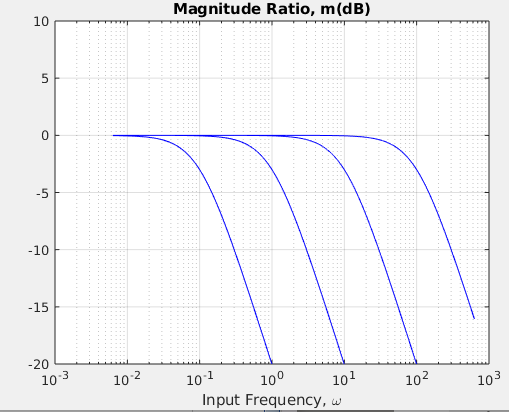
\includegraphics[scale=.30]{images/lecture2_fig7.png}
				This is a Bode plot. It seems abstract but there is some very useful information shown.\vspc

				  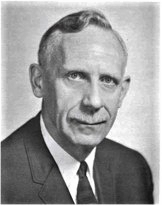
\includegraphics[scale=.4]{images/hendrikbode.png} \vspc Hendrik Bode (1905-1982) 

				\end{multicols}
								
				\btVFill 
			\end{frame}

			\begin{frame}
				\frametitle{\sectionIIsubsectionIIItitle}
				\bigskip

				
				\btVFill 
			\end{frame}

			
		% section II subsection IV
		\subsection{\sectionIIsubsectionIVtitle}\label{sectionIIsubsectionIV}

			\begin{frame}[containsverbatim]
				\frametitle{\sectionIIsubsectionIVtitle}
				\bigskip

				\frametitle{Bode Plot in MATLAB}

				MATLAB has a built it tool for making Bode plots.  
				\begin{multicols}{2}
				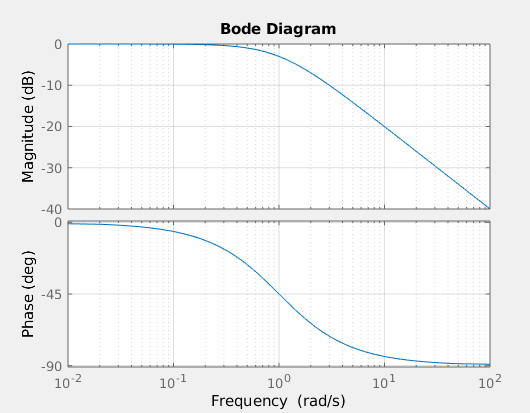
\includegraphics[scale=.25]{images/lecture2_fig9.png}

				\begin{lstlisting}
				figure(1)
				sys=tf(1,[tau(3) 1])
				bode(sys);grid on
				\end{lstlisting}

				\end{multicols}

				So what? What can you do with a Bode diagram?
								
				\btVFill 
			\end{frame}	

			\begin{frame}
				\frametitle{\sectionIIsubsectionIVtitle}
				\bigskip

				\frametitle{References}

				\begin{itemize}
					\item System Dynamics, Palm III, Third Edition - Chapter 9 - System Response in the Frequency Domain
				\end{itemize}
				

				\btVFill 
			\end{frame}	
		
	% Section III
	\section{\sectionIIItitle}\label{sectionIII}

		% section III Outline
		\begin{frame}
			\large \textbf{Topic 3 - \sectionIIItitle} \vspace{3mm}\\

			\begin{itemize}
				\item \hyperlink{sectionIIIsubsectionI}{\sectionIIIsubsectionItitle} \vspc %  section III subsection I
				\item \hyperlink{sectionIIIsubsectionII}{\sectionIIIsubsectionIItitle} \vspc % section III subsection II
				\item \hyperlink{sectionIIIsubsectionIII}{\sectionIIIsubsectionIIItitle} \vspc % section III subsection III
				\item \hyperlink{sectionIIIsubsectionIV}{\sectionIIIsubsectionIVtitle} \vspc % section III subsection IV
			\end{itemize}

		\end{frame}

		% section III subsection I
		\subsection{\sectionIIIsubsectionItitle}\label{sectionIIIsubsectionI}

			\begin{frame}
				\frametitle{\sectionIIIsubsectionItitle}
				\bigskip

				\frametitle{Equivalent System Representations}

				\small 
				The{\bf Transfer Function} is the input-output relationship in the frequency domain and can be found from the equation of motion of the system.\vspcc 

				\scalebox{1.25}{$T(s)=\frac{X(s)}{F(s)}$}\vspcc

				The Transfer Function is an equivalent representation of the system. \vspcc
				\begin{framed}
				\scalebox{1.25}{E.O.M$\hspace{5mm} \leftrightarrow \hspace{5mm}$ T(s)$\hspace{5mm} \leftrightarrow \hspace{5mm}$ Block Diagram}\\
				\end{framed}

				\btVFill
			\end{frame}

			\begin{frame}
				\frametitle{\sectionIIIsubsectionItitle}
				\bigskip

				\frametitle{Transfer Function of 2$^{nd}$ Order System}

				\scalebox{1}{$m\ddot{x}+c\dot{x}+kx=f(t)$ \hspace{5mm}with\hspace{5mm} $f(t)=Asin(\omega t)$} \vspcc
				The transfer function can easily be found by taking the Laplace transform of the equation of motion. \vspcc

				\begin{framed}
				\scalebox{1}{$T(s)=\frac{X(s)}{F(s)}=\frac{1}{ms^2+cs+k}$ \hspace{5mm} Second Order Transfer Function} \vspc
				\end{framed}

				\btVFill
			\end{frame}

		% section III subsection II
		\subsection{\sectionIIIsubsectionIItitle}\label{sectionIIIsubsectionII}	

			\begin{frame}
				\frametitle{\sectionIIIsubsectionIItitle}
				\bigskip
				\frametitle{The Overdamped System}

				\small

				In an \underline{overdamped} system, both roots are real and distinct.\vspcc
				The transfer function is shown below in terms of the system parameters\vspc

				\scalebox{1.0}{$T(s)=\frac{X(s)}{F(s)}=\frac{1/k}{\left(\frac{m}{k}\right)s^2+\left(\frac{c}{k}\right)s+1}=\frac{1/k}{(\tau_1 s+1)(\tau_2 s+1)} \hspace{5mm} \tau_1,\tau_2$ - time constants}\vspc

				Substitute $s=j\omega$ into the transfer function and find the amplitude ratio and phase angle.\vspc

				\scalebox{1.0}{$T(s) \rightarrow T(j\omega) =\frac{1/k}{\left(\tau_1j\omega+1\right)\left(\tau_1j\omega+1\right)}$}\vspc

				\begin{framed}
				\scalebox{1}{$M\left(\omega\right)=|T\left(j\omega\right)|=\frac{|1/k|}{|\tau_1j\omega+1||\tau_2j\omega+1|}$} \vspc
				\scalebox{1}{$m\left(\omega\right)=20logM\left(\omega\right)=20log|1/k|-20log|\tau_1\omega j+1|-20log|\tau_2\omega j+1|$}\vspc
				\scalebox{1}{$\phi\left(\omega\right)=\angle\frac{1}{k}-\angle\left(\tau_1\omega j+1\right)-\angle\left(\tau_2\omega_j+1\right)$}
				\end{framed}

				\btVFill
			\end{frame}

			\begin{frame}
				\frametitle{\sectionIIIsubsectionIItitle}
				\bigskip

				\frametitle{The Bode Diagram}
				\small
				These three terms can be seen on the Bode diagram. \vspc
				\scalebox{1}{$m\left(\omega\right)=20logM\left(\omega\right)=20log|1/k|-20log|\tau_1\omega j+1|-20log|\tau_2\omega j+1|$}\vspc

				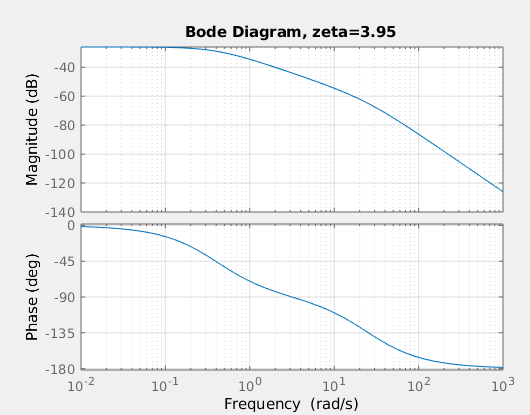
\includegraphics[scale=.30]{images/lecture3_fig3.png}

				This shows that the magnitude ratio of the system across different regions of the input frequency. 

				\btVFill
			\end{frame}

		% section III subsection III
		\subsection{\sectionIIIsubsectionIIItitle}\label{sectionIIIsubsectionIII}

			\begin{frame}
				\frametitle{\sectionIIIsubsectionIIItitle}
				\bigskip

				\frametitle{The Underdamped System}

				\small

				In an \underline{underdamped} system, the roots are complex conjugates.\vspcc
				The transfer function is shown below in terms of the system parameters\vspc

				\scalebox{1.0}{$T(s)=\frac{X(s)}{F(s)}=\frac{1/k}{\left(\frac{m}{k}\right)s^2+\left(\frac{c}{k}\right)s+1}=\frac{1/k}{\left(\frac{s}{\omega_n}\right)^2+2\zeta\left(\frac{s}{\omega_n}\right)+1}$} \vspc
				\scalebox{1.0}{$T(s)=\frac{kX(s)}{F(s)}=\frac{\omega_n^2}{s^2+2\zeta\omega_ns+\omega_n^2}$}\vspc

				Notice we factored out $k$ to form the ratio of output displacement $X(s)$ to input displacement $\frac{F(s)}{k}$. You can see this with Hooke's Law $F=kx\implies x=\frac{F}{k}$. \vspc

				This also allows us to define the transfer function in terms of $\zeta$ and $\omega_n$. Substitue $s=j\omega$ and mulitply the equation $\frac{1/\omega_n^2}{1/\omega_n^2}$.
				\scalebox{1.0}{$T(s)\rightarrow T(j\omega)=\frac{1}{\left(\frac{j\omega}{\omega_n}\right)^2+\left(\frac{2\zeta}{\omega_n}\right)j\omega+1}=\frac{1}{1-\left(\frac{\omega}{\omega_n}\right)^2+\left(\frac{2\zeta\omega}{\omega_n}\right)j}$} \vspc
	
				\btVFill
			\end{frame}

			\begin{frame}
				\frametitle{\sectionIIIsubsectionIIItitle}
				\bigskip

				\frametitle{The Frequency Ratio}

				\small 

				To simplify this expression we define another new quantity the frequency ratio, $r$ as the ratio of input frequency to natural frequency of the system. The transfer function is re-written in terms of the frequency ratio. \vspc

				\scalebox{1.0}{$r=\frac{\omega}{\omega_n} \hspc\rightarrow\hspc T\left(j\omega\right) \hspc\rightarrow\hspc T\left(r\right)=\frac{1}{1-r^2+2\zeta rj}$} \vspcc

				Now the amplitude ratio and phase are written in tems of $r$. \vspcc

				\begin{framed}
				\scalebox{1}{$M=|T\left(r\right)|=\frac{1}{\sqrt{\left(1-r^2\right)^2+\left(2\zeta r\right)^2}}$}\vspc
				\scalebox{1}{$\implies m=20logM=-10log\left[\left(1-r^2\right)^2+\left(2\zeta r\right)^2\right]$} \vspcc
				\scalebox{1}{$\phi=\angle 1 - \angle\left(1-r^2+2\zeta rj\right)\implies \phi=-tan\left(\frac{2\zeta r}{1-r^2}\right)$}\vspc
				\end{framed}

				\btVFill
			\end{frame}

			\begin{frame}
				\frametitle{\sectionIIIsubsectionIIItitle}
				\bigskip

				\frametitle{The Bode Diagram}
				\small

				In the underdamped second order system only two regions are present in the Bode diagram. 

				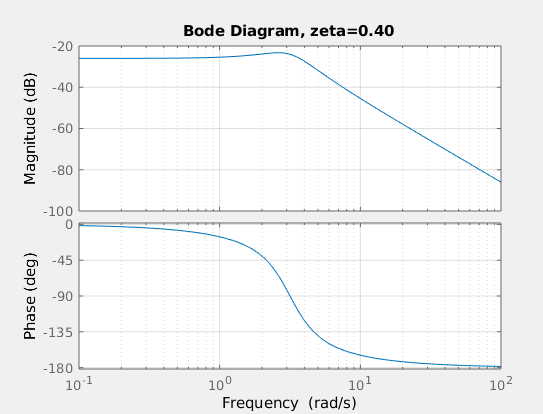
\includegraphics[scale=.27]{images/lecture3_fig4.png}  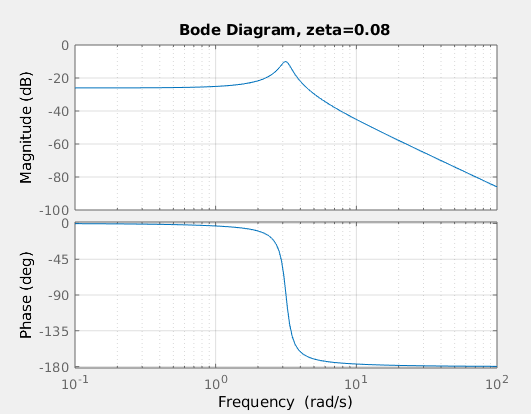
\includegraphics[scale=.27]{images/lecture3_fig5.png} 

				As the damping ratio decreases something significant happens. This Bode diagram shows something that the others before have not.

				\btVFill
			\end{frame}

		% section III subsection IV
		\subsection{\sectionIIIsubsectionIVtitle}\label{sectionIIIsubsectionIV}	

			\begin{frame}[containsverbatim]
				\frametitle{\sectionIIIsubsectionIVtitle}
				\bigskip

				Vary the system parameter in the scripts to make the plots shown. 

				\begin{lstlisting}
				clear variables;clc;close all

				% define the system parameters
				m=2;c=1;k=20;
				zeta=c/(2*sqrt(m*k));

				% create a system object from the transfer function
				sys=tf(1/k,[(m/k) (c/k) 1]);

				% use built-in MATLAB Bode Plot
				figure(1)

				bode(sys);grid on
				str=sprintf('Bode Diagram, zeta=%.2f',zeta);
				title(str)
				\end{lstlisting}

				\btVFill 
			\end{frame}

			\begin{frame}
				\frametitle{\sectionIIIsubsectionIVtitle}
				\bigskip

				\frametitle{References}

				\begin{itemize}
					\item System Dynamics, Palm III, Third Edition - Chapter 9 - System Response in the Frequency Domain
				\end{itemize}
			
		 		\btVFill 
			\end{frame}

	% Section IV
	\section{\sectionIVtitle}\label{sectionIV}

		% section IV Outline
		\begin{frame}
			\large \textbf{Topic 3 - \sectionIVtitle} \vspace{3mm}\\

			\begin{itemize}
				\item \hyperlink{sectionIVsubsectionI}{\sectionIVsubsectionItitle} \vspc %  section III subsection I
				\item \hyperlink{sectionIVsubsectionII}{\sectionIVsubsectionIItitle} \vspc % section III subsection II
				\item \hyperlink{sectionIVsubsectionIII}{\sectionIVsubsectionIIItitle} \vspc % section III subsection III
				\item \hyperlink{sectionIVsubsectionIV}{\sectionIVsubsectionIVtitle} \vspc % section III subsection IV

			\end{itemize}

		\end{frame}

		% section IV subsection I
		\subsection{\sectionIVsubsectionItitle}\label{sectionIVsubsectionI}

			\begin{frame}
				\frametitle{\sectionIVsubsectionItitle}
				\bigskip

				\frametitle{Transfer Function of 2$^{nd}$ Order System}

				\scalebox{1}{$m\ddot{x}+c\dot{x}+kx=f(t)$ \hspace{5mm}with\hspace{5mm} $f(t)=Asin(\omega t)$} \vspcc
				The transfer function can easily be found by taking the Laplace transform of the equation of motion. \vspcc

				\begin{framed}
				\scalebox{1}{$T(s)=\frac{X(s)}{F(s)}=\frac{1}{ms^2+cs+k}$ \hspace{5mm} Second Order Transfer Function} \vspc
				\end{framed}

				The amplitude ratio and phase angle can be found from the transfer function. Think about what $M$ means. \vspc

				\btVFill
			\end{frame}

			\begin{frame}
				\frametitle{\sectionIVsubsectionItitle}
				\bigskip

				\frametitle{Overdamped vs. Underdamped Systems}

				\small

				In an \underline{overdamped} system, both roots are real and distinct.\vspc

				\begin{framed}
				\scalebox{0.75}{$M\left(\omega\right)=|T\left(j\omega\right)|=\frac{|1/k|}{|\tau_1j\omega+1||\tau_2j\omega+1|}$} \vspc
				\scalebox{0.75}{$m\left(\omega\right)=20logM\left(\omega\right)=20log|1/k|-20log|\tau_1\omega j+1|-20log|\tau_2\omega j+1|$}\vspc
				\scalebox{0.75}{$\phi\left(\omega\right)=\angle\frac{1}{k}-\angle\left(\tau_1\omega j+1\right)-\angle\left(\tau_2\omega_j+1\right)$}
				\end{framed}
				In an \underline{underdamped} system, the roots are complex conjugates.\vspc
				\begin{framed}
				\scalebox{0.75}{$M\left(r\right)=|T\left(r\right)|=\frac{1}{\sqrt{\left(1-r^2\right)^2+\left(2\zeta r\right)^2}}$ \hspc with \hspc$r=\frac{\omega}{\omega_n} $}\vspc
				\scalebox{0.75}{$\implies m=20logM=-10log\left[\left(1-r^2\right)^2+\left(2\zeta r\right)^2\right]$} \vspc
				\scalebox{0.75}{$\phi=\angle 1 - \angle\left(1-r^2+2\zeta rj\right)\implies \phi=-tan\left(\frac{2\zeta r}{1-r^2}\right)$}\vspc
				\end{framed}
				
				\btVFill
			\end{frame}

		% section IV subsection II
		\subsection{\sectionIVsubsectionIItitle}\label{sectionIVsubsectionII}	

			\begin{frame}
				\frametitle{\sectionIVsubsectionIItitle}
				\bigskip

				\frametitle{The Resonance Spike}

				In the underdamped second order system only two regions are present separated by the point near $r=1$. \vspc

				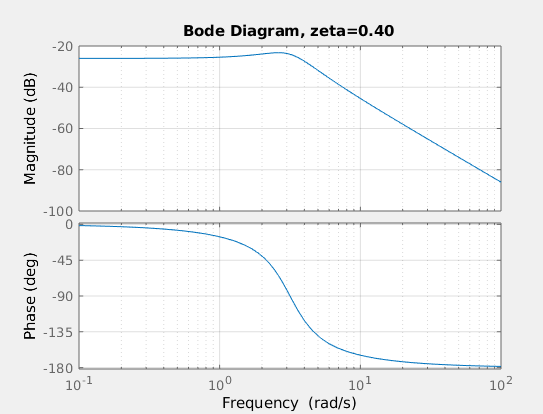
\includegraphics[scale=.18]{images/lecture4_fig1.png} 
				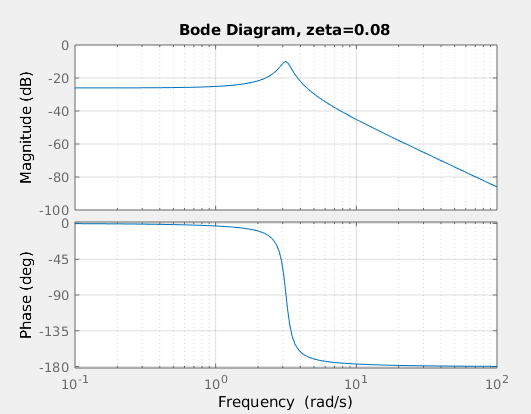
\includegraphics[scale=.18]{images/lecture4_fig2.png} 
				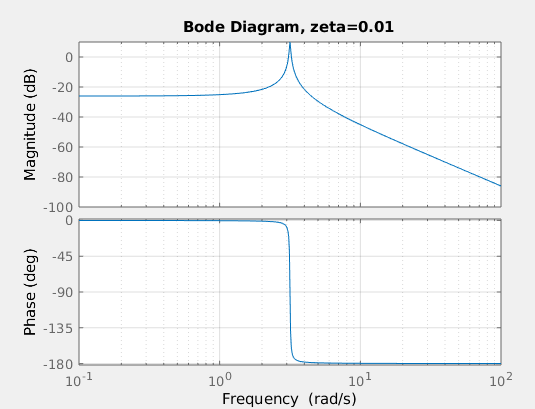
\includegraphics[scale=.18]{images/lecture4_fig3.png}  \vspc

				As the damping ratio decreases something significant happens at this points. Remember, these are graphs of $m=20logM$. \vspc
	
				\btVFill
			\end{frame}

			\begin{frame}
				\frametitle{\sectionIVsubsectionIItitle}
				\bigskip

				\frametitle{The Effects of Resonance}

				\small

				Consider the extreme case in the figure shown. What is the physical significance of the values of $m$ near $r=1$?  \vspc
				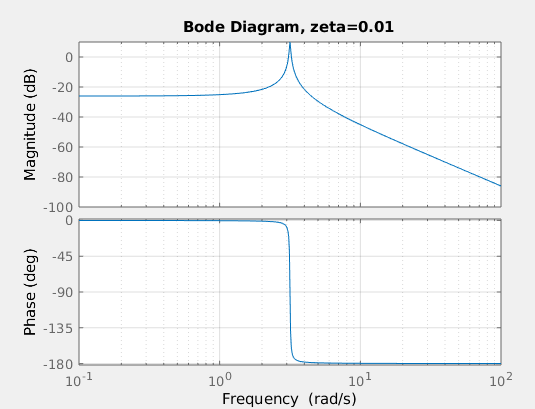
\includegraphics[scale=.25]{images/lecture4_fig3.png}\hspace{10mm} 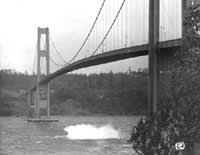
\includegraphics[scale=.6]{images/galloping_gertie_02.jpg}  \vspc

				\btVFill
			\end{frame}

			\begin{frame}
				\frametitle{\sectionIVsubsectionIItitle}
				\bigskip

				\frametitle{The Effects of Resonance}

				\small

				Consider the extreme case in the figure shown. What is the physical significance of the values of $m$ near $r=1$?  \vspc
				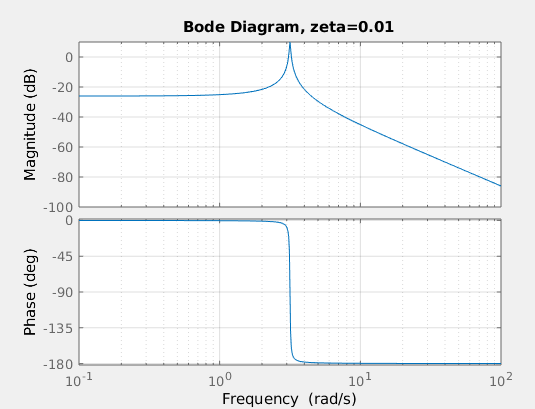
\includegraphics[scale=.25]{images/lecture4_fig3.png}\hspace{10mm} 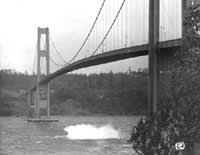
\includegraphics[scale=.6]{images/galloping_gertie_02.jpg}  \vspc

				\btVFill
			\end{frame}

		% section IV subsection III
		\subsection{\sectionIVsubsectionIIItitle}\label{sectionIVsubsectionIV}

			\begin{frame}
				\frametitle{\sectionIVsubsectionIIItitle}
				\bigskip

				\frametitle{Resonance can be Destructive}

				\small

				The resonance peak represents a amplitude  ratio greater than one meaning the output amplitude is larger that in the input amplitude. This large amplitude output displacement caused by resonance correspond to a large force in the spring members and the large forces are transmitted to the body. Large forces cause mechanical failure.

				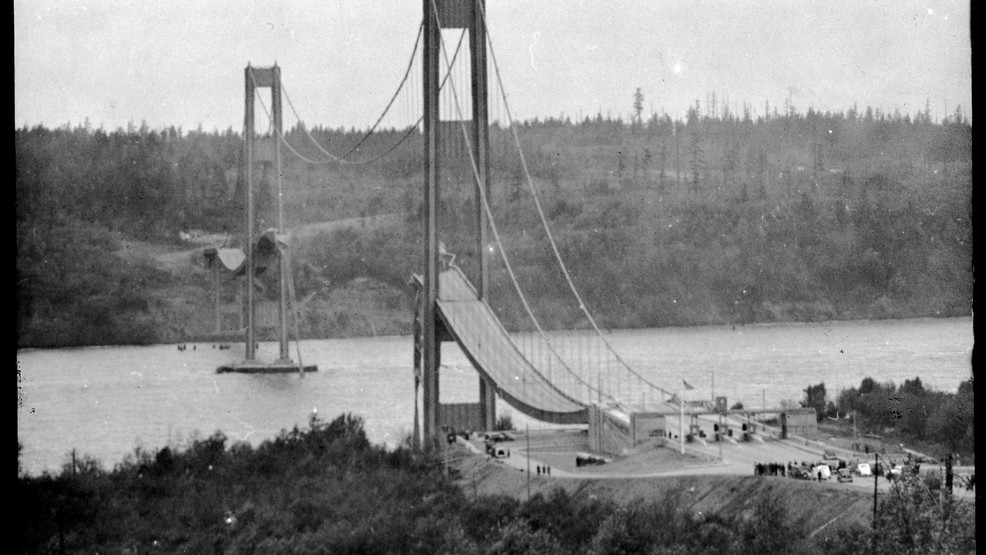
\includegraphics[scale=.20]{images/galloping_gertie_01.jpg}  \vspc

			
				\btVFill
			\end{frame}

			\begin{frame}
				\frametitle{\sectionIVsubsectionIIItitle}
				\bigskip

				Where on the frequency response graphs does resonance occur? It looks like it is {\it near} $r=1$.\vspc

				\scalebox{1}{$M\left(r\right)=\frac{1}{\sqrt{\left(1-r^2\right)^2+\left(2\zeta r\right)^2}}$ \hspc with \hspc$r=\frac{\omega}{\omega_n}$}\vspc

				The value of $M$ is maximized when the denominator is minimized. Therefore the resonance frequency is found by taking the derivative of the denominator and setting it equal to zero.  \vspc

				\scalebox{1}{$M_{max}$ \hspc occurs at $r=\sqrt{1-2\zeta^2} \implies \omega=\omega_n\sqrt{1-2\zeta^2} $}\vspc

				An input frequency equal to the resonance frequency causes maximum output displacement.  \vspc

				\btVFill
			\end{frame}

			\begin{frame}
				\frametitle{\sectionIVsubsectionIIItitle}
				\bigskip

				\frametitle{The  Resonance Frequency}
				The resonance event only occurs in second order systems when the radical shown is positive. This corresponds to systems with damping ratio in the range $0<\zeta< 0.707$ . \vspc

				\scalebox{1}{$\omega_r=\omega_n\sqrt{1-2\zeta^2} \hspc 0<\zeta< 0.707$} \vspc

				\scalebox{1}{$M_r=\frac{1}{2\zeta\sqrt{1-\zeta^2}}$\hspccc or in decibels\hspccc$m_r=-20log\left(2\zeta\sqrt{1-\zeta^2}\right)$} \vspc

				The phase at resonance can also be found. \vspc

				\scalebox{1}{$\phi_r=tan^{-1}\left(\frac{\sqrt{1-2\zeta^2}}{\zeta}\right)$}\vspc

				\btVFill
			\end{frame}

			\begin{frame}
				\frametitle{\sectionIVsubsectionIIItitle}
				\bigskip

				It is important to note that we multiplied the transfer function by $k$ during the derivations. Therefore if me divide the expressions for $M$ and $M_r$ by $k$ to find the amplitude ratio between input force, $f(t)$ and output displacement, $x_{ss}(t)$\vspc

				\scalebox{1}{$M=\frac{1}{k\sqrt{\left(1-r^2\right)^2+\left(2\zeta r\right)^2}}$}\vspc
				\scalebox{1}{$\implies \hspcc m=-20log(k)-10log\left[\left(1-r^2\right)^2+\left(2\zeta r\right)^2\right]$}\vspc
				\scalebox{1}{$M_r=\frac{1}{k2\zeta\sqrt{1-\zeta^2}}$}\vspc
				\scalebox{1}{$\implies \hspcc m_r=-20log\left(k\right)-20log\left(2\zeta\sqrt{1-\zeta^2}\right) $}\vspc

				\btVFill
			\end{frame}

			\begin{frame}
				\frametitle{\sectionIVsubsectionIIItitle}
				\bigskip

				\frametitle{References}

				\begin{itemize}
					\item System Dynamics, Palm III, Third Edition - Chapter 9 - System Response in the Frequency Domain
				\end{itemize}

				\btVFill
			\end{frame}

		% section IV subsection IV
		\subsection{\sectionIVsubsectionIVtitle}\label{sectionIVsubsectionIV}	

			\begin{frame}
				\frametitle{\sectionIVsubsectionIVtitle}
				\bigskip



				

				\btVFill 
			\end{frame}

			\begin{frame}
				\frametitle{\sectionIVsubsectionIVtitle}
				\bigskip

			

		 		\btVFill 
			\end{frame}
			
			\begin{frame}
				\frametitle{\sectionIVsubsectionIVtitle}
				\bigskip
				
				
					
				\btVFill 
			\end{frame}

			\begin{frame}
				\frametitle{\sectionIVsubsectionIVtitle}
				\bigskip
			
				
				\btVFill 
			\end{frame}



\end{document}





